\section{Regler}
\subsection{Schaltenderegler}
\subsubsection{Zweipunkte-Regler}\script{64}
Ein Zweipunktregler ist ein unstetig arbeitender Regler mit zwei Ausgangszuständen. Je nachdem,
ob der Istwert über oder unter dem Sollwert liegt, wird der erste oder der zweite Ausgangszustand
eingenommen.

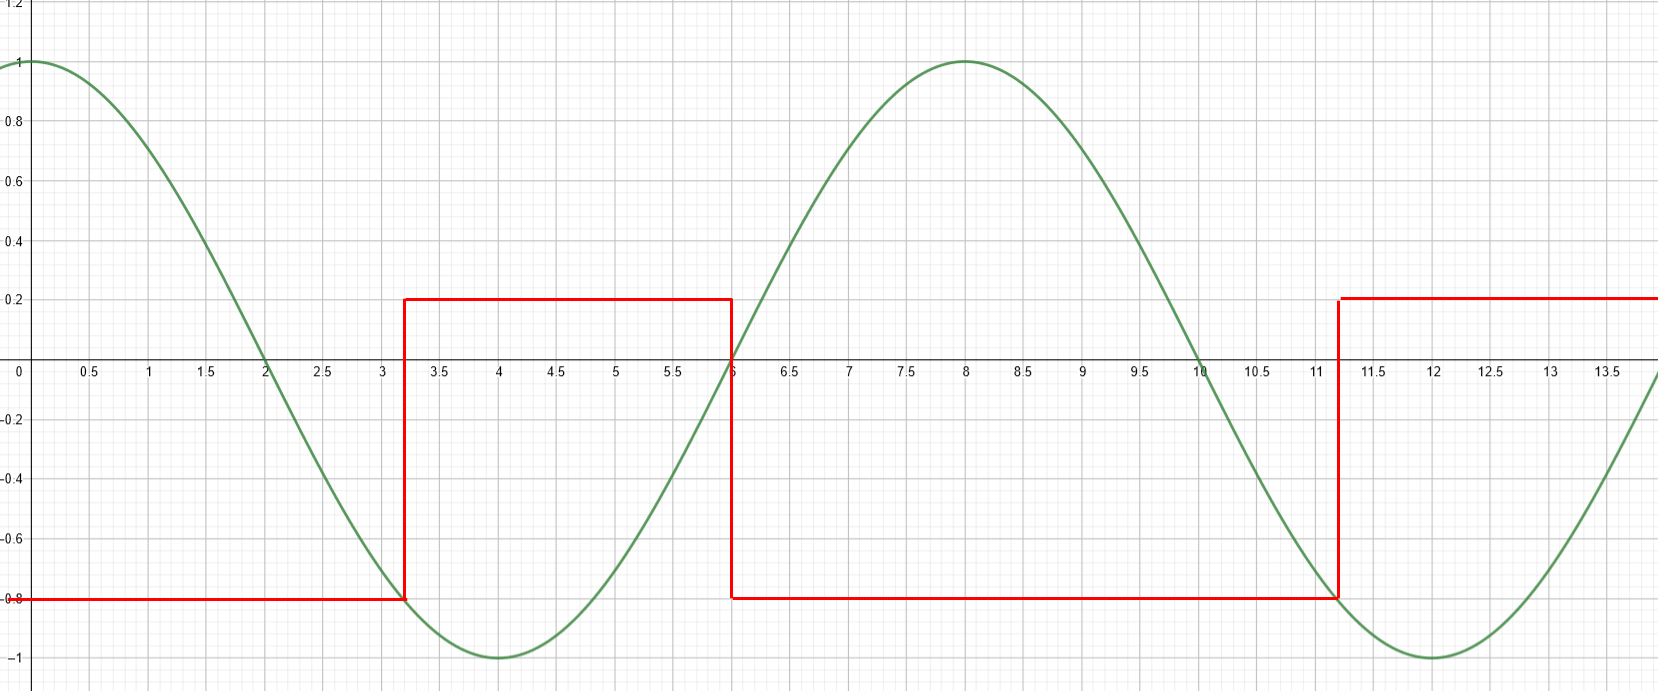
\includegraphics[width=\columnwidth,keepaspectratio=true]{Images/zweipunkte-regler}\\
Linke Kurve zeigt \textcolor{red}{oberer}, Rechte Kurve \textcolor{green}{untere} Grenze an. Vorteil dieses Reglers, er ist sehr einfach zu implementieren, hat aber keinen stabilen Zustand.

\subsubsection{Dreipunkt-Regler}\script{70}
Im Gegensatz zum Zweipunktregler gibt es im Dreipunktregler eine Ruhelage. Dies ist eine Kompination aus zwei Zweipunktregler.\\
\begin{center}
	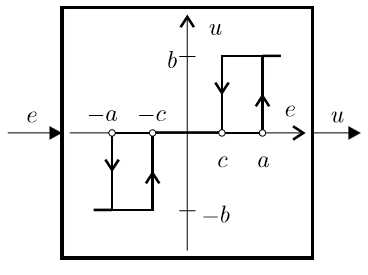
\includegraphics[width=0.3\columnwidth]{Images/dreipunktregler}
\end{center}

\textbf{Beispiel Konvertierung}
\begin{center}
	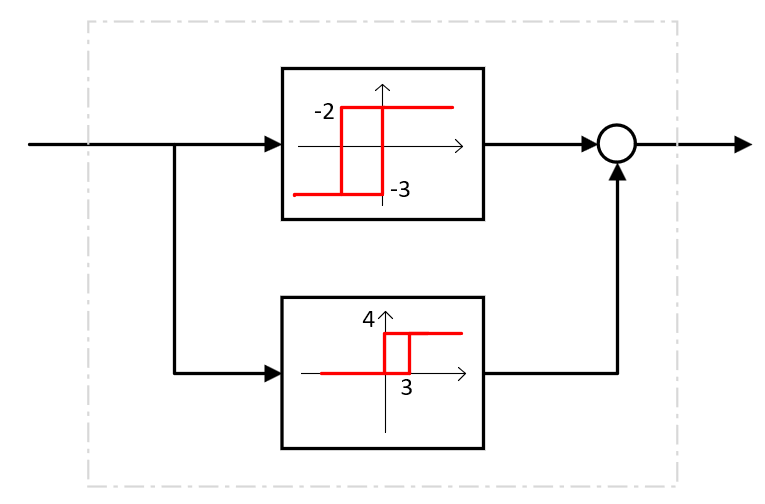
\includegraphics[width=0.5\columnwidth]{Images/3pr_I}
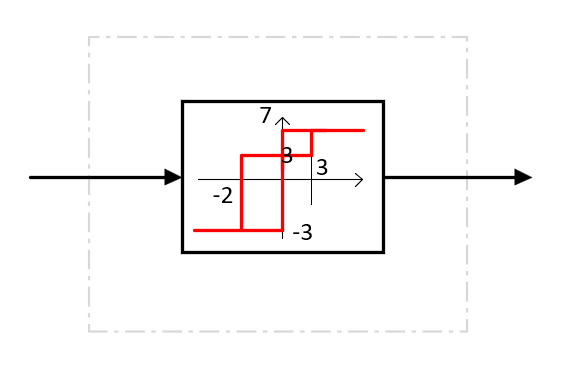
\includegraphics[width=0.4\columnwidth]{Images/3pr_II}
\end{center}


\subsection{Stetigähnlicher Regler}\script{71}
Sind spezielle Regler, welche modifizierte Schaltenderegler sind. Gegenüber schaltenden Reglner sind stetigähnliche Regler also aufwendiger zu bauen, aber am Regerausgang ändert sich nicht viel.